\documentclass[a4paper]{article}
\usepackage{authblk}
\usepackage[pdftex]{graphicx}
\usepackage{sidecap}
\usepackage[T1]{fontenc}
\usepackage[utf8]{inputenc}
\usepackage[magyar]{babel}
\usepackage{hyperref}
\sloppy
\usepackage{listings}
\lstset{language=C++}

\author[1]{András~Mamenyák}
\author[1]{Roland~Bamli}
\affil[1]{Mérnök informatikus (BSc) szakos hallgató, Debreceni Egyetem}

\title{Neurális hálózatok alkalmazása spam szűrésre}

\begin{document}
\maketitle

\section{Neurális hálózatok}
\subsection{A neurális hálózatok kialakulása}
A neurális hálózatok a mesterséges inteligencia egy típusa, amelyet az állatok központi idegrendszere, különösen az agy ihletett, amely képes a tanulásra, a mintafelismerésre is. Megalkotásához biológiai ismeretekre és az idegsejt működésének pontosabb megismerésére volt szükség. Ez csak a 20. században valósult meg. Az első neuron modelt 1947-ben alkotta meg McCullock és Pitts, az első mesterséges neuront pedig Rosenblatt 1958-ban. A neurális hálózatok egy ígéretes, új tudományterület, mely Webos 1974-es "back propagation" algoritmusa és annak 1986-os újra felfedezése után indult igazán fejlődésnek.

\subsection{A mesterséges neuron felépítése, működése}
Egy mesterséges neuron, mint a biológiai, több bemenettel és egy kimenettel rendelkezik (\ref{artifical_neuron}. ábra). Egy általános neuron működése szerint  meghatározza a bemenetek súlyozott összegét és ezen végrehajt valamilyen nem lineáris leképezést. Ez utóbbit nevezik aktivációs, transzfer vagy aktiváló függvénynek. A végeredmény pedig a neuron kimeneti jele. Egy másik változat a lineráris összegzést megvalósító neuron, amikor nem történik lineáris leképezés.

\begin{figure}
  \centering
  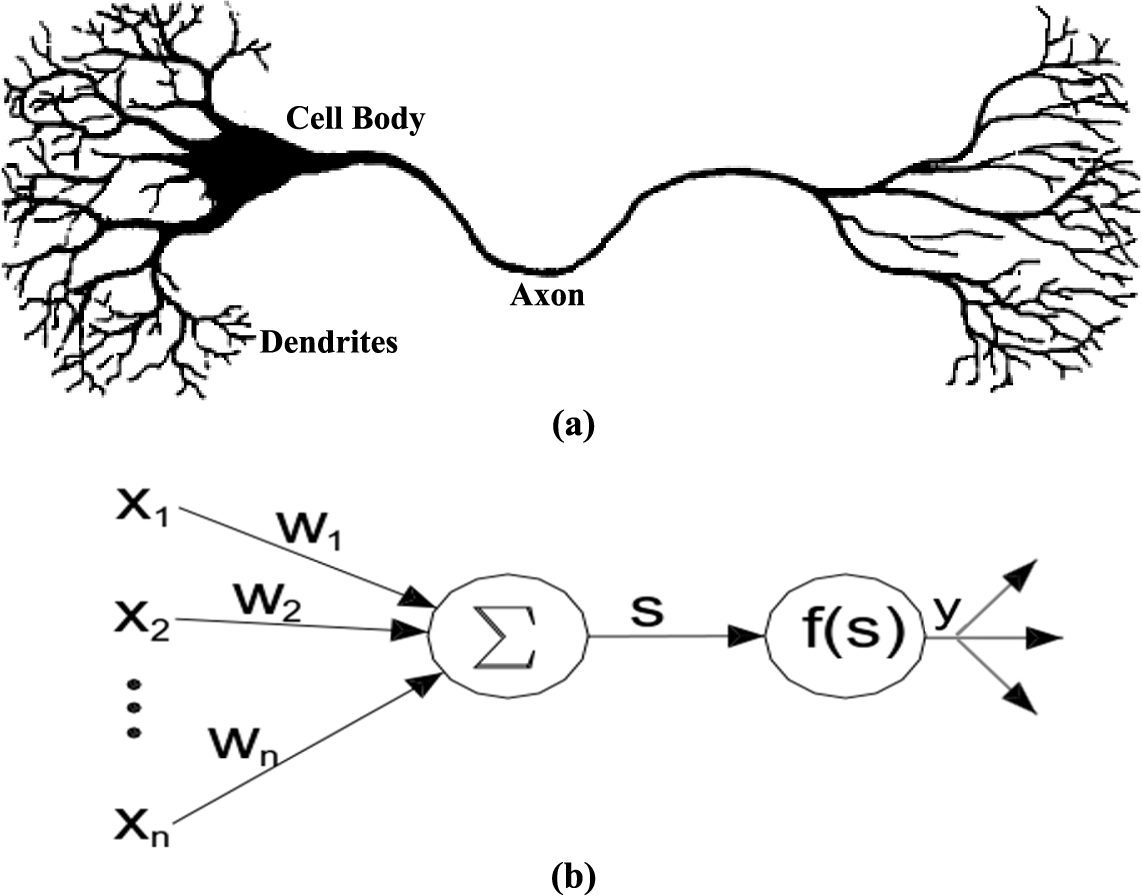
\includegraphics[scale=0.6]{artifical_neuron}
  \caption{A biológiai neuron (a) és a mesterséges neuron (b) összehasonlítása}
  \label{artifical_neuron}
\end{figure}

A \ref{artifical_neuron}. ábrán a neuron bemeneteit x${_i}$ jelöli, a kimeneti jel pedig y. Először a bemenetek súlyozott összegei kerülnek meghatározásra: $${s=\sum_{i=0}^{n} W_i \cdot x_i = W^T \cdot x}$$

Abban az esetben, ha a neuron lineáris összegzést valósít meg, ezzel már meg is kaptuk a kimeneti jelet:$${y = s = W^T \cdot x}$$

Nem lineáris esetben szükség van még a nem lineáris leképezésre. Ebben az esetben a neuron kimeneti jele a következő:$${y = f(s) = f(W^T \cdot x)}$$ ahol ${f(s)}$ az aktivizációs függvény. Erre a célra a négy leggyakrabban használt függvény a lépcső- vagy szignumfüggvény, a ``telítéses lineáris'' függvény, a tangens hiperbolikusz függvény és a szigmoid függvény.

Használnak egy másik elterjedt neuron típust is a RBF (Radial Bass Function) hálózatokban. Ennél a típusnál nincs lineáris összegzés,  az összes bemenet az aktivizációs függvénybe kerül, mely több bemenet esetén több változós függvény lesz.

\subsection{A neuron hálózatok felépítése}
A neuronokból álló hálózatokat nevezzük neurális hálózatoknak. Ezekben minden neuron ugyanolyan, vagy hasonló műveleteket végez, a többi neurontól függetlenül, lokálisan. Tehát ezek a hálózatok olyan információfeldolgozó eszközök, amelyek párhuzamos, elosztott működésre, tanulásra képesek. Általában irányított gráffal reprezentáljuk őket. A neuronok a gráf csomópontjai, míg a gráf élei a kimenetek és bemenetek közötti kapcsolatot reprezentálják. Megvalósíthatók szoftveresen, hardveresen, vagy a kettő kombinációjaként is. 

A neuronok három fajtáját különböztetjük meg:
\begin{enumerate}
    \item\textbf{bemeneti neuronok:} Egy bemenetű, egy kimenetű, buffer jellegű neuronok, jelfeldolgozó feladatuk nincs. Bemenetük a hálózat bemenete, kimenetük más neuronok meghajtására szolgál.
    \item\textbf{rejtett neuronok:} Ezek a neuronok végzik a jelfeldolgozást. Kimenetük és bemenetük is más neuronokhoz csatlakozik.
    \item\textbf{kimeneti neuronok:} A környezet felé továbbítják kimenetüket.
\end{enumerate}

A neuronokat álltalában típusa alapján rétegekbe szervezzük. Ennek megfelelően beszélhetünk bemeneti rétegről, retjett réteg(ek)ről és kimeneti rétegről.

A neuronhálózatokat az egyes neuronok közötti összeköttetési rendszer alapján két fő csoportba sorolhatjuk. Beszélhetünk előrecsatolt hálózatokról (\ref{forward_neuron}. ábra) és visszacsatolt hálózatokról. 

\subsection{Előrecsatolt (Feedforward) hálózatok}

\begin{figure}
  \centering
  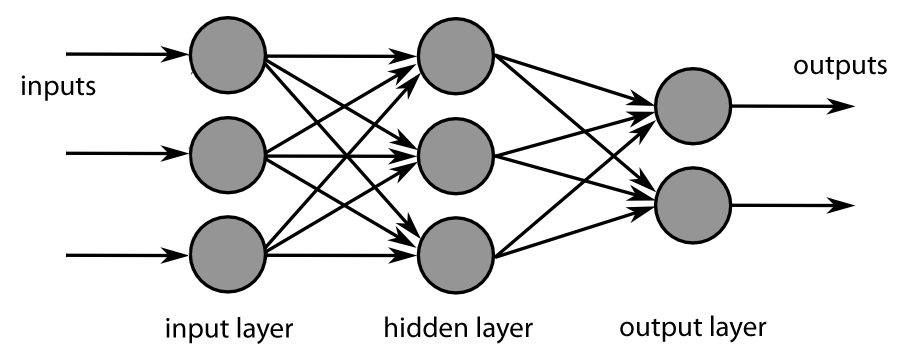
\includegraphics[scale=0.3]{neuron_layers}
  \caption{Előrecsatolt neuron hálózatok felépítése.}
  \label{forward_neuron}
\end{figure}

Az előrecsatolt hálózatokban a jel csak egy irányba terjedhet, a bemeneti rétegtől, a rejtett rétegeken át,  a kimeneti réteg felé. Nincsen visszacsatolás (hurok), a neuronok kimenete nincs hatással arra rétegre, amelyben találhatóak. Széles körben használják minta felismerésre.

\subsubsection{Single-layer Perceptron hálózatok}
A Perceptron hálózatok a legegyszerűbb neurális hálózatok, melyekben a bemeneti réteg neuronjai közvetlenül a kimeneti réteghez csatlakoznak. A hálózat a Perceptron algoritmus szerint működik, melyet 1957-ben dolgozott ki Frank Rosenblatt. Jellemzői:
\begin{itemize}
    \item\textbf{képes megtanulni egyszerű minták felismerését} 
    \item\textbf{kétrétegű:} az input rétegnek csak elosztó szerepe van, Perceptronok valójában csak egy rétegben vannak
    \item\textbf{folyamatos értékű és bináris inputtal egyaránt működhet}
    \item\textbf{offline módon tanul, időciklusokban működik}
    \item\textbf{egy perceptron azt dönti el, hogy egy input minta két osztály közül melyikhez tartozik.}
    \item\textbf{felügyelt tanulást végez}
\end{itemize}

\begin{figure}
  \centering
  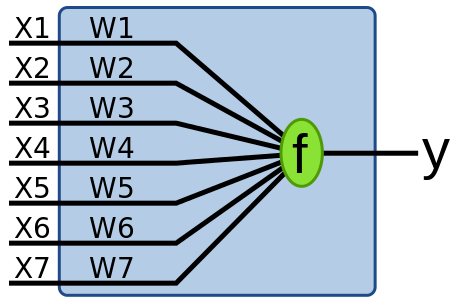
\includegraphics[scale=0.3]{Perceptron}
  \caption{Egy Perceptron hálózatbeli neuron működése.}
  \label{forward_neuron}
\end{figure}

Az algoritmus a működése a során a bemeneti jelek ($x_{i}$) és a hozzájuk tartozó súlyok ($w_{i}$) alapján számolja ki a hálózat kimenetét. Az alábbi képlet szerint:
$${ n = f(\sum_{i=0}^{m} x_{i}w_{i})},$$

ahol
\[ f(x) = \left\{
  \begin{array}{l l}
    1, & \quad \textrm{ha $x > t$}\\
    0, & \quad \textrm{egyébként}
  \end{array} \right.\]

A hálózat inicializálásakor meg kell adnunk a súlyok kezdőértékét és a $t$ (threshold) értékét. A súlyoknak vagy 0-t, vagy véletlenszerűen választott kis érteket érdemes adni. Ezen kívül értéket kell adnunk még $r$-nek (learning rate). Ez egy 0 és 1 közé eső szám lehet. Amennyiben túl nagyra választjuk, a peceptron ingadozni fog a megoldás körül.

Miután megvan a hálózat kimenete ($n$), a várt kimenetből ($z$), kiszámoljuk a hibát ($e$):
$$e = z - n$$

Ezután a korrigálást:
$$d = r * e $$

Végül frissítjük a súlyokat:
$$w_{i} = w_{i} + d * x_{i}$$

Amikor a hiba értéke 0, nem változtatunk a súlyokon. A tanulási folyamat akkor ér véget, ha a egyik train bemenetre sem kell változtatni a súlyokon, vagyis a hálózat mindegyikre a várt eredményt adja.

\subsubsection{Többrétegű előrecsatolt hálózatok}
Ezekben a hálózatokban több számítást végző réteg található meg. Minden egyes neuron kimenete a következő rétegre van kapcsolva. A többrétegű hálózatoknál több tanuló algoritmus közül is választhatunk, a legelterjedtebb a back-propagation algoritmus.
\subsubsection{Back-propagation algoritmus}
A back-propagation, teljes nevén ``backward propagation of errors'', magyarul hiba-visszaterjesztési eljárás, egy tanulási algoritmus, melyet gyakran használnak a neurális hálózatokban. Ez egy felügyelt tanulási módszer, melynek szüksége van egy nagy adatbázisra a bemenetekkel és a kívánt kimenetekkel. Alkalmazása az előrecsatolt hálózatoknál a leghasznosabb. Használatához meg kell követelnünk, hogy a neuron hálózat réteges felépítésű, a neuron átviteli függvénye pedig deriválható legyen.A tanítás alapgondolata, hogy az elvárt és a számított kimenetek eltérését, mint a háló súlyaitól függõ hibát értelmezzük és ezen, a súlyok terében értelmezett hibafüggvényen hajtunk végre egy minimális pont keresést. Az algoritmusban a tanulás lényegében a hátrafelé terjedés folyamata, mely során minimalizálni kell az elvárt és a tényleges output vektor közötti négyzetes eltérést, Euklideszi távolságot.

Működése alapján két fázisra lehet osztani, terjedésre (propagation) és a súlyok frissítésére. A terjedés során a jel mind előre, mind hátra a szinapszisok és a neuronok szintjén lokális információk alapján terjed. A súlyok frissítése a neuron kimenetére visszaérkezett jel alapján történik (\ref{backpropagation}. ábra).

\begin{figure}
  \centering
  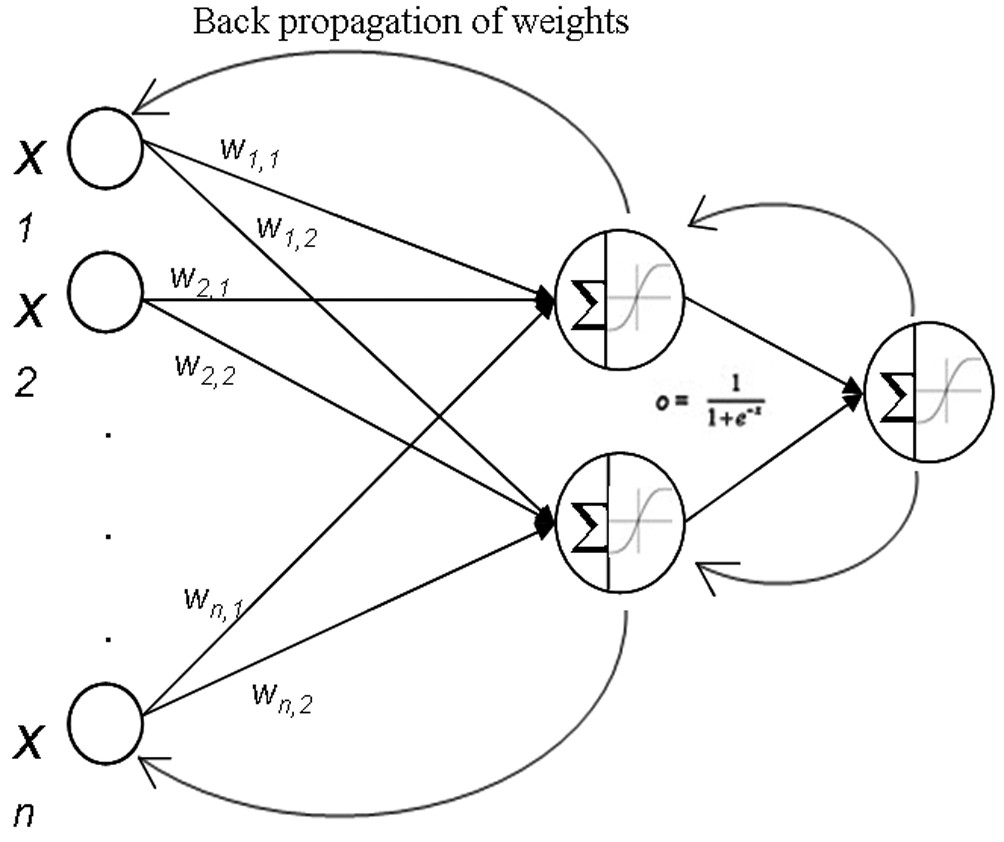
\includegraphics[scale=0.8]{backpropagation}
  \caption{A back-propagation algoritmus működése.}
  \label{backpropagation}
\end{figure}


\subsection{Visszacsatolt (Recurrent) hálózatok}
Akkor nevezünk egy neurális hálózatot visszacsatoltnak, ha a topológiáját reprezentáló irányított gráf tartalmaz hurkot. Ez esetben beszélhetünk globális és lokális visszacsatolásról.

\begin{itemize}
    \item\textbf{elemi visszacsatolás (recurrent connections):} egy réteg egy neuronjának kimenete közvetlenül egyik saját bemenetére van visszacsatolva,
    \item\textbf{laterális visszacsatolás (lateral connections):} valamely réteg(ek) neuronjainak kimenetei ugyanazon réteg neuronjainak bemeneteire kapcsolódnak, de nem értjük ide a neuron önmagára való visszacsatolását.
    \item\textbf{rétegek közötti visszacsatolás (inter-layer connections):} több réteget tartalmazó hurkot hoznak létre a gráfon.
\end{itemize}

\section{Spam szűrés}
\subsection{Bevezetés}
Az elektronikus üzenetküldés nagyon fontos részévé vált a mindennapi életnek. Egy olyan részévé, mely segítségével ingyen és egyszerűen küldhetünk üzeneteket a világ bármely pontjára. Sajnos ezeknek az üzeneteknek egy része kéretlenül érkezik, ezeket nevezzük spam üzeneteknek. Bizonyára mindenkit zavarnak az ilyen üzenetek, de különösen a vállalatok számára okoznak növekvő problémát, illetve jelentős anyagi kárt. A spam üzenetek következményei:
\begin{itemize}
    \item\textbf{idő veszteség}
    \item\textbf{tárhely veszteség}
    \item\textbf{fontos üzenet elvesztése}
    \item\textbf{hálózat túlterhelése} 
    \item\textbf{rosszindulatú programok}  
\end{itemize}

\noindent
A spam szűrési techinkákat működésük alapján így csoportosíthatjuk:
\begin{itemize}
    \item\textbf{lista alapú szűrők:} Blacklist, Whitelist,
    \item\textbf{tartalom alapú szűrők:} Word-Based Filters, Heuristic Filters, Bayesian Filters
    \item\textbf{egyébb szűrők:} DNS Lookup System, Challenge/Response System
\end{itemize}

\subsection{Neurális hálózatok alkalmazása}
A neurális hálózatokat nem olyan olyan széles körben elterjedtek, mint például a Bayes-szűrés. Ennek oka lehet, hogy a Bayes-szűrés elég egyszerű, mégis nagyon jó hatékonysággal működik. A neurális hálózatoknak nagyobb az erőforrás igénye, és több mintára van szüksége.

A hálózat működéséhez szükség van minta üzenetekre. Ezekről tudnunk kell, hogy spamek-e, a tanulás folyamán ugyanis ezek lesznek a várt kimenetek (1 ha spam, 0 ha nem). A bemeneti paramétereket az üzenetek szövegéből kell kiszámítanunk. Ezek alapján hasonlítja majd össze a neurális hálózat az üzeneteket és ez alapján próbálja spam és nem spam csoportokra bontani.

\end{document}